\section{Defining Evolvability}

\begin{frame}{Defining Evolvability}
consensus: the amount of useful variation generated by the evolutionary process
\begin{itemize}
  \item evolvability as the ability to generate heritable variation
  \item evolvability as bias towards useful variation
\end{itemize}
\end{frame}

% \begin{frame}{The Evolvability Conundrum}
% How can natural selection ``favor properties hat may prove useful to a given lineage in the future, but have no present adaptive function''? \cite{Pigliucci2008IsEvolvable}
% \end{frame}


\subsection{Evolvability as Heritable Variation}

\begin{frame}{Evolvability as Heritable Variation}
	\begin{figure}
 \centering
    \begin{subfigure}[b]{0.5\textwidth}
        \centering
    	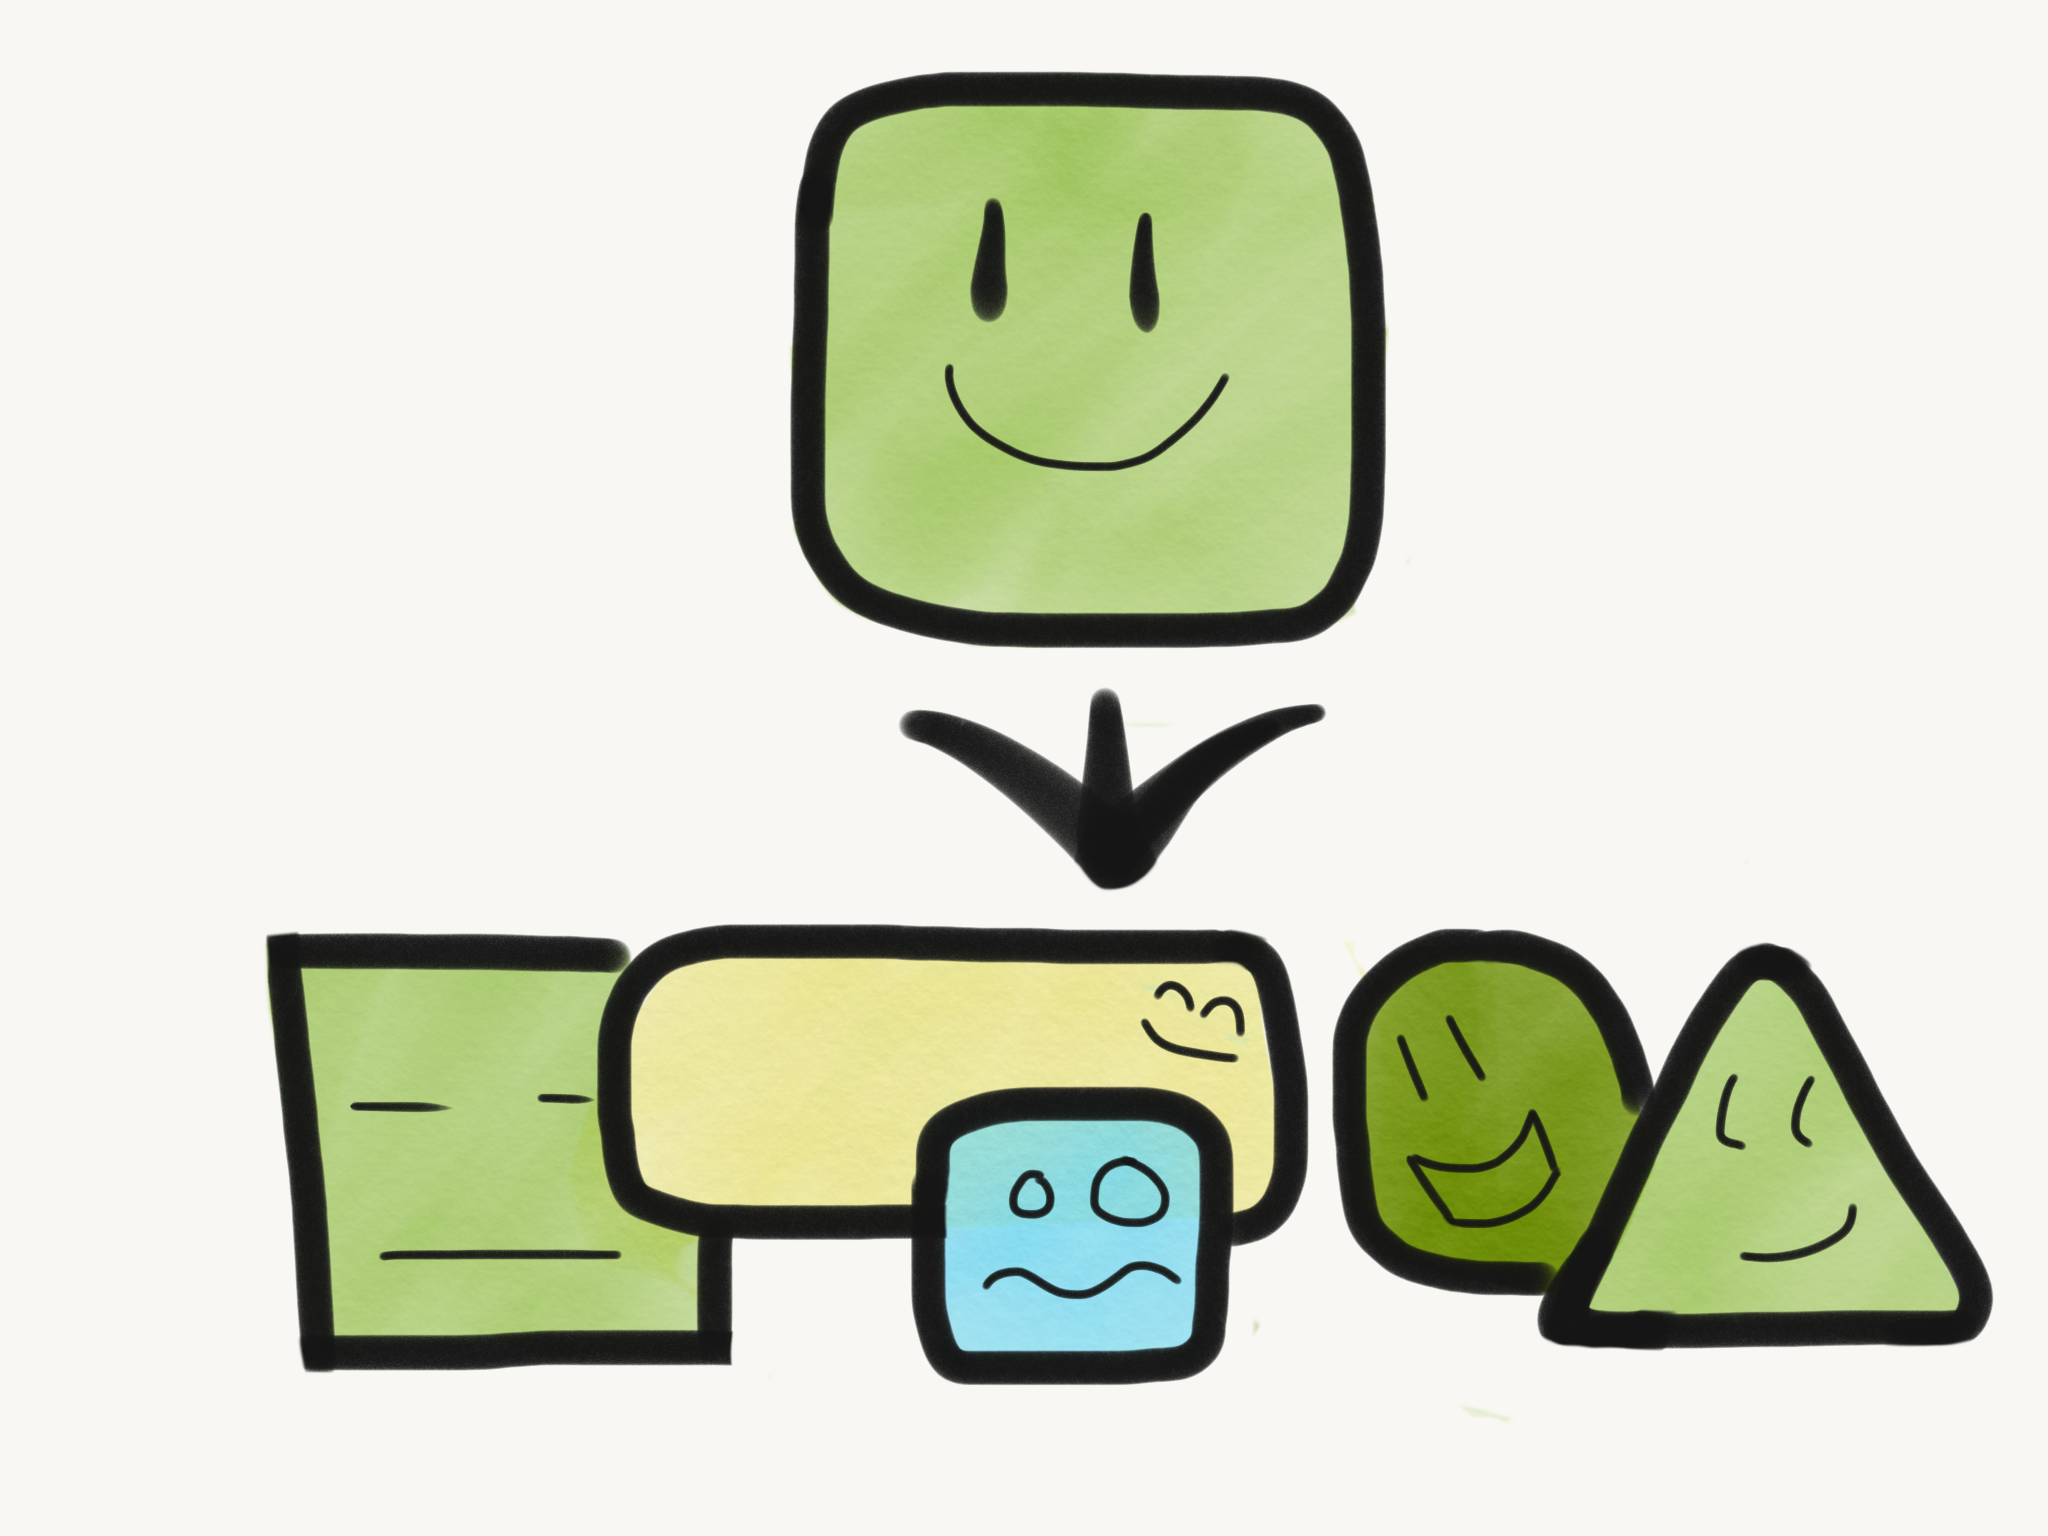
\includegraphics[width=\textwidth]{img/individual_evolvability.png}
        \caption{high individual evolvability}
        \label{subfig:canalization}
    \end{subfigure}%
    \hfill
    \begin{subfigure}[b]{0.5\textwidth}
        \centering
        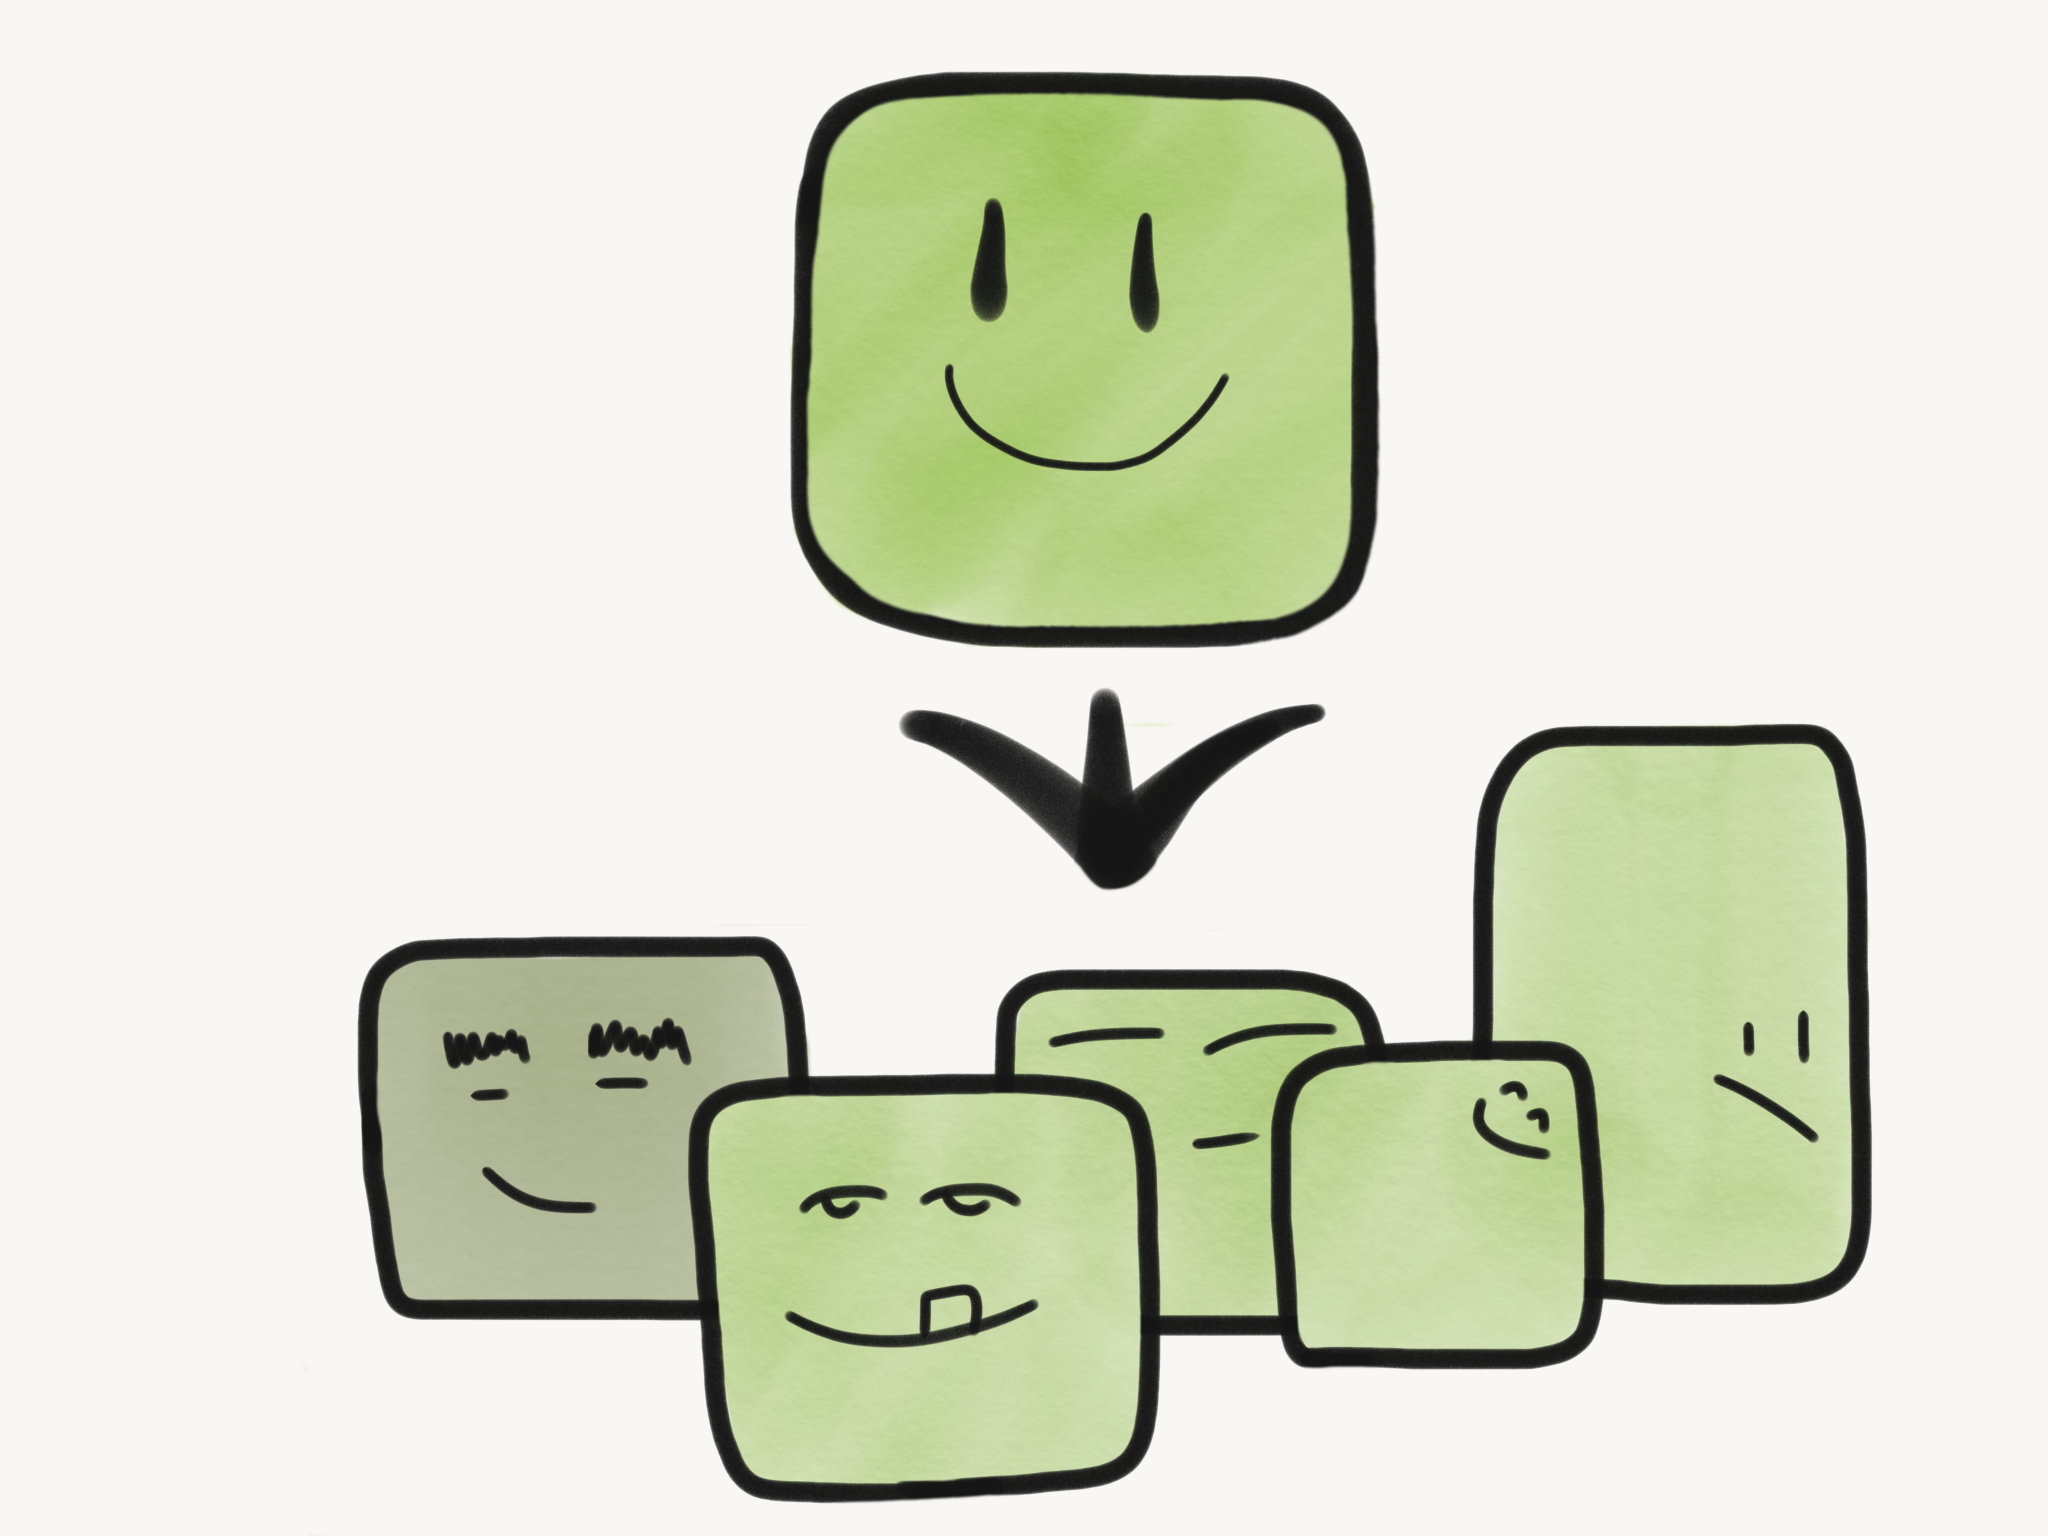
\includegraphics[width=\textwidth]{img/low_individual_evolvability.png}
        \caption{low individual evolvability}
        \label{subfig:no_canalization}
    \end{subfigure}
 	\captionsetup{singlelinecheck=off,justification=raggedright}
    \vspace{-4ex}
  \captionsetup{singlelinecheck=off,justification=raggedright}
  \caption{An illustration of individual evolvability, considering evolvability as heritable variation \cite{Wilder2015ReconcilingEvolvability}.}
  \label{fig:high_vs_low_individual_evolvability}
\end{figure}
\end{frame}

\begin{frame}{Evolvability as Heritable Variation}
  \begin{figure}
 \centering
    \begin{subfigure}[b]{0.5\textwidth}
        \centering
    	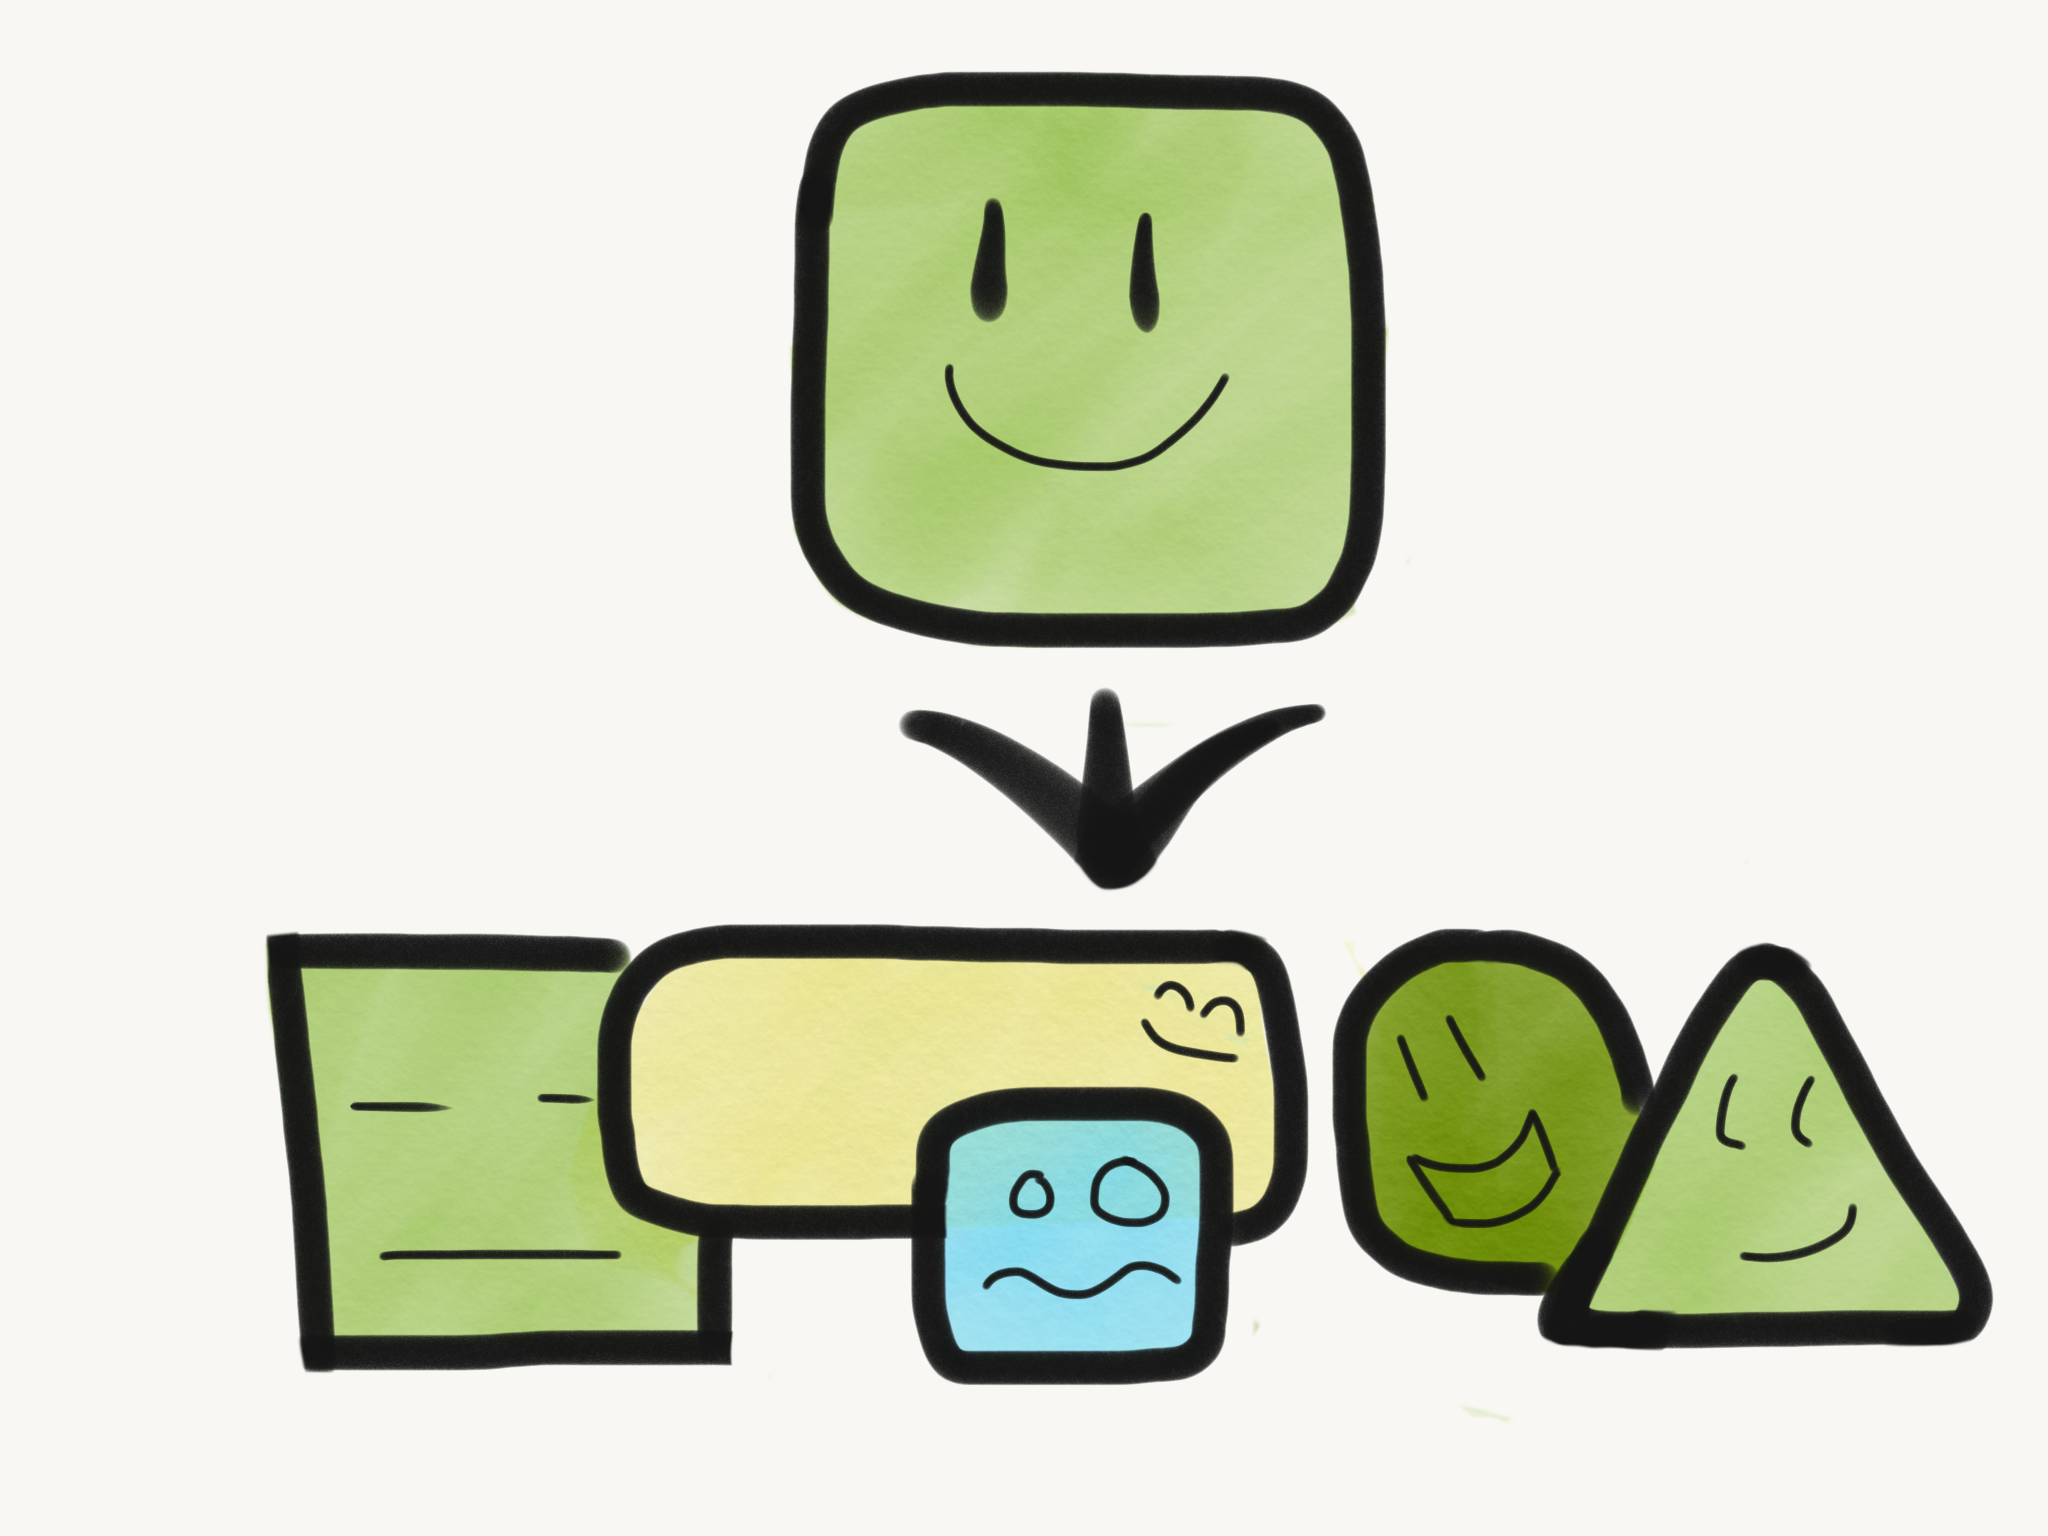
\includegraphics[width=\textwidth]{img/individual_evolvability}
        \caption{individual evolvability}
        \label{subfig:individual_evolvability}
    \end{subfigure}%
    \hfill
    \begin{subfigure}[b]{0.5\textwidth}
        \centering
        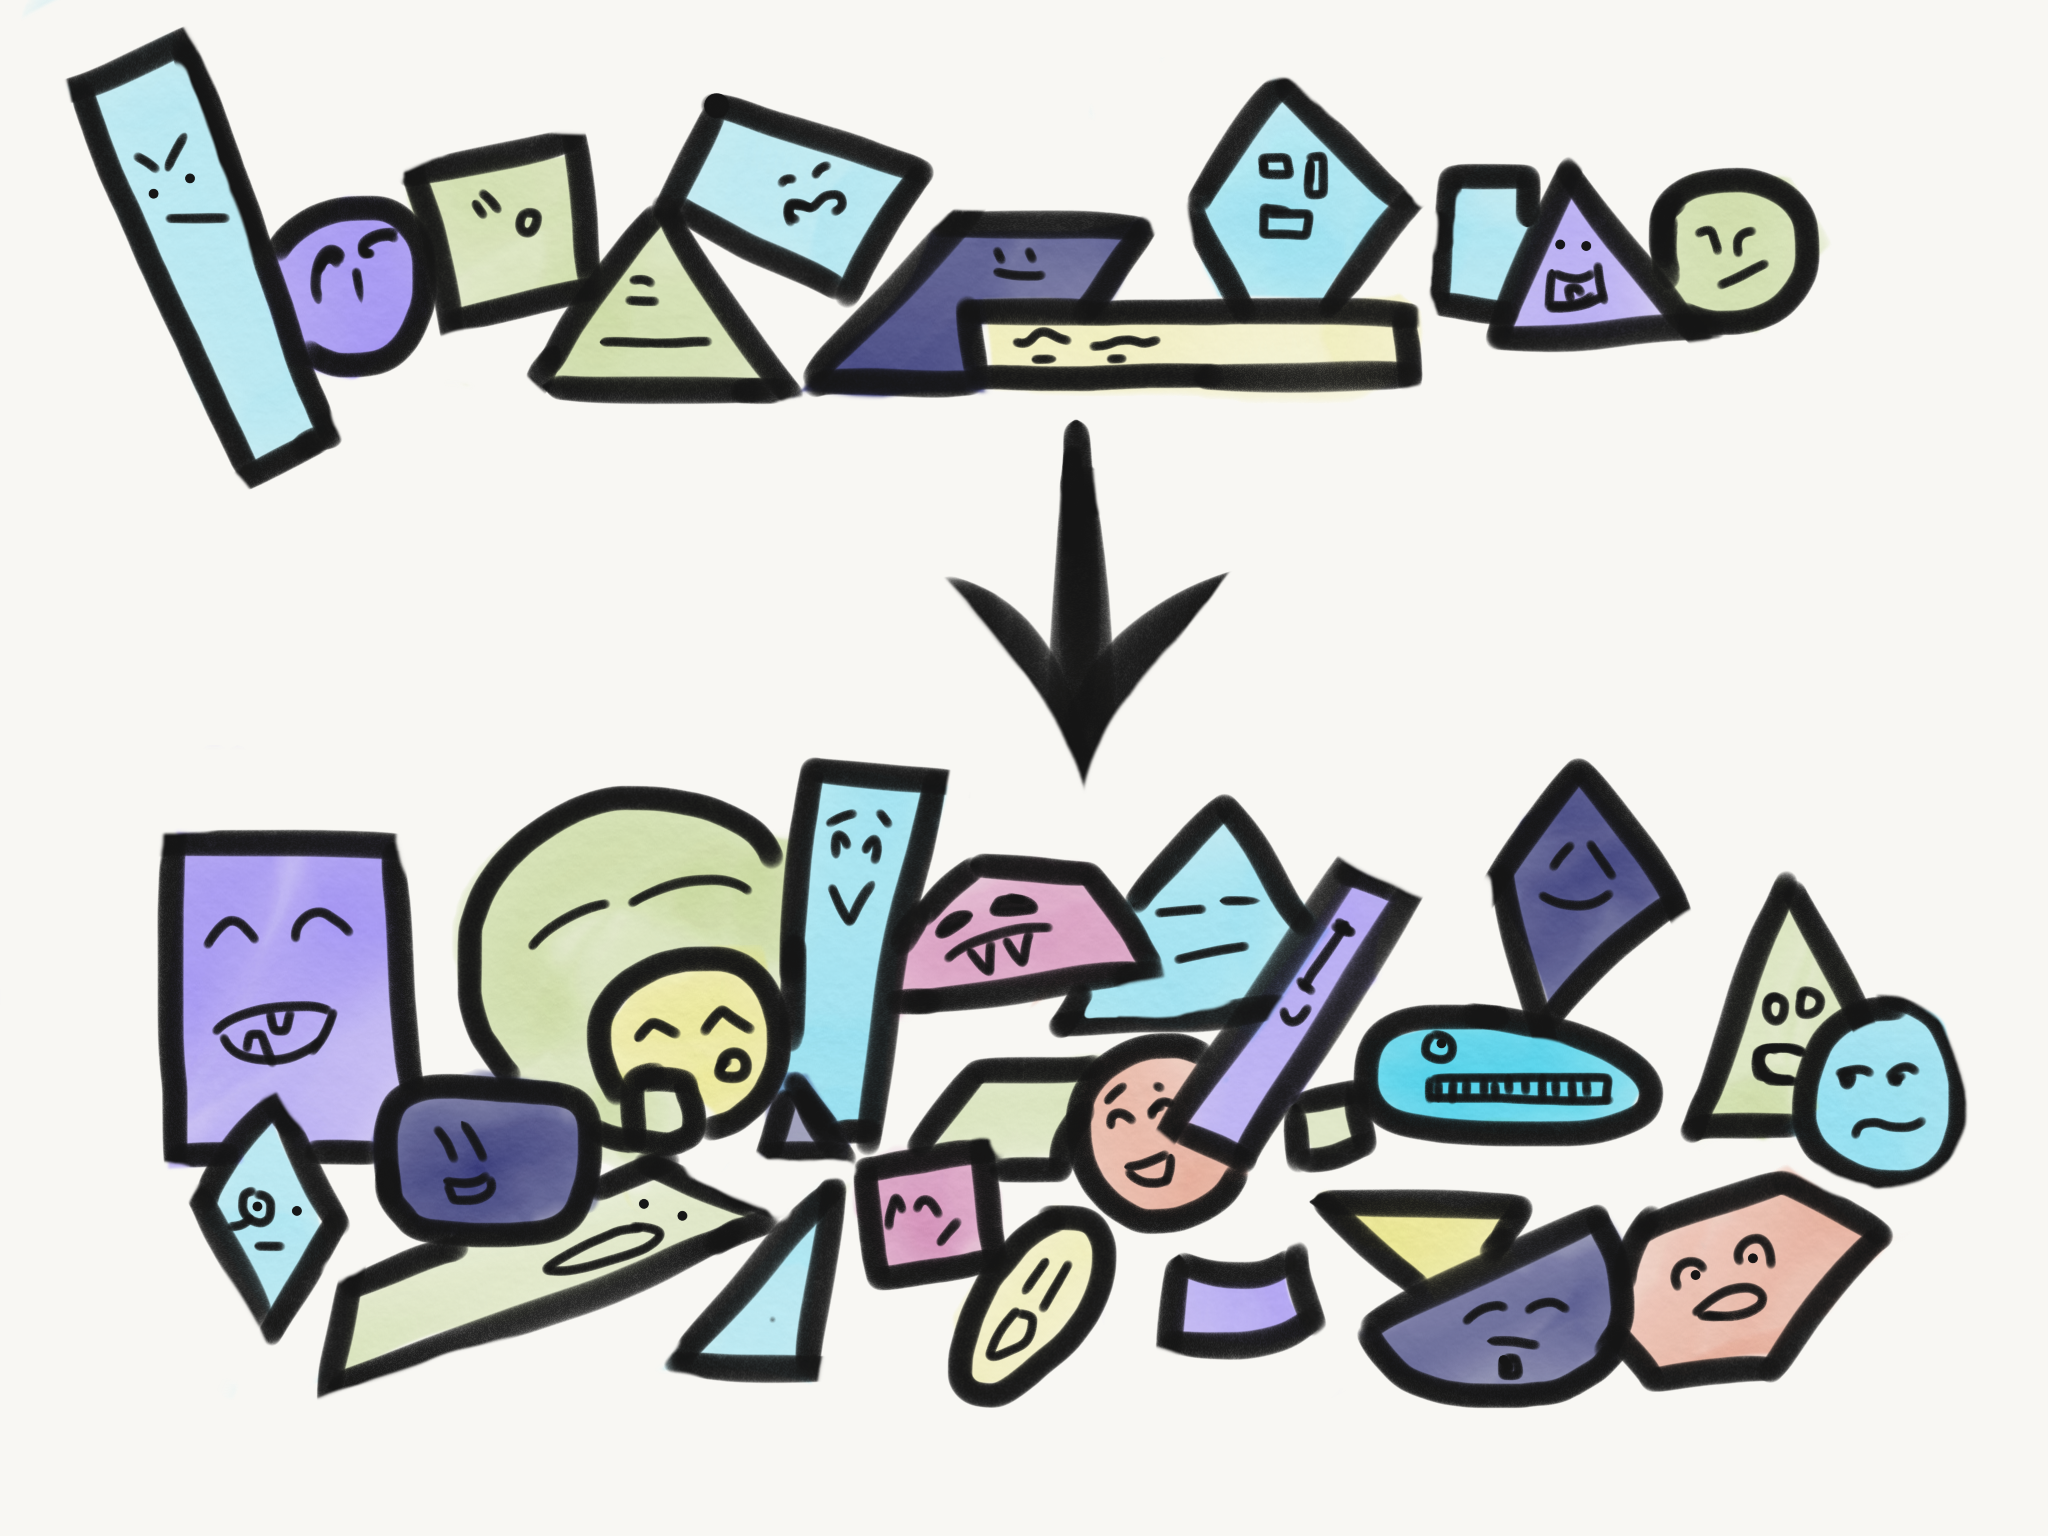
\includegraphics[width=\textwidth]{img/population_evolvability}
        \caption{population evolvability}
        \label{subfig:population_evolvability}
    \end{subfigure}
 	\captionsetup{singlelinecheck=off,justification=raggedright}
    \vspace{-4ex}
  \captionsetup{singlelinecheck=off,justification=raggedright}
  \caption{An illustration contrasting individual and population evolvability \cite{Wilder2015ReconcilingEvolvability}.}
  \label{fig:individual_vs_population_evolvability}
\end{figure}
\end{frame}

\subsection{Evolvability as Bias towards Useful Variation}

\begin{frame}{Evolvability as Bias towards Useful Variation}
  \begin{figure}
    \centering
    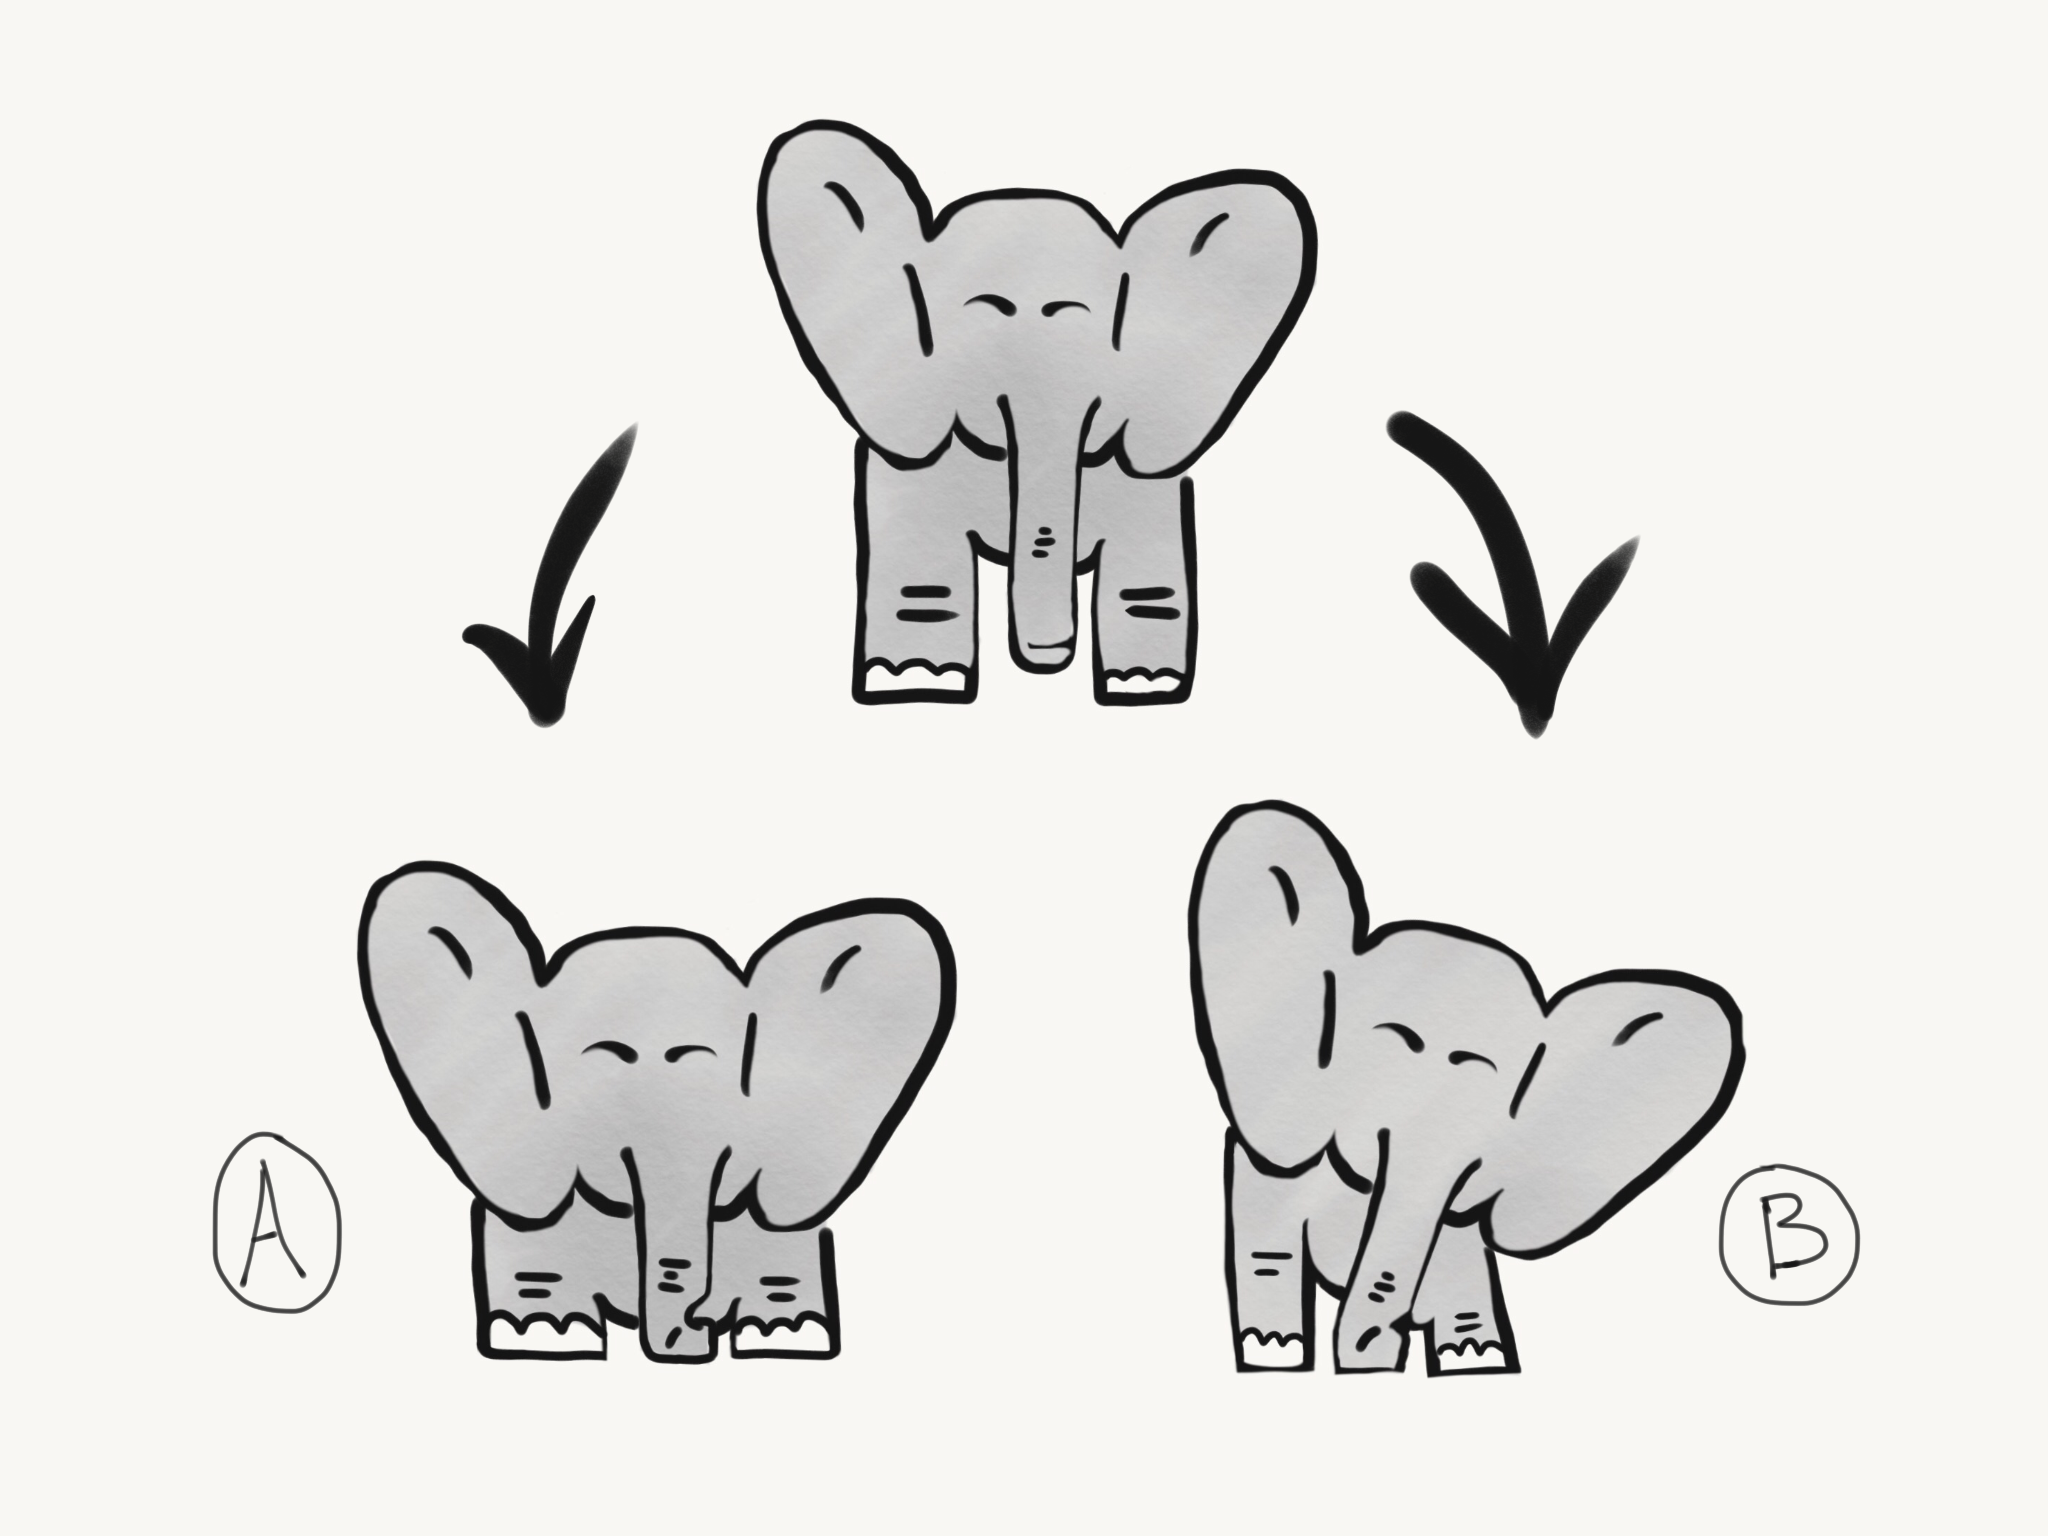
\includegraphics[width=0.8\textwidth]{img/developmental_constraint}
 	\captionsetup{singlelinecheck=off,justification=raggedright}
  	\caption{Illustration of developmental constraint; high evolvability left and low evolvability right \cite{Smith1985DevelopmentalBiology,Tuinstra1990LackDevelopment}.}
    \label{fig:developmental_constraint}
\end{figure}
\end{frame}

\begin{frame}{Evolvability as Bias towards Useful Variation}
  \begin{figure}
    \centering
    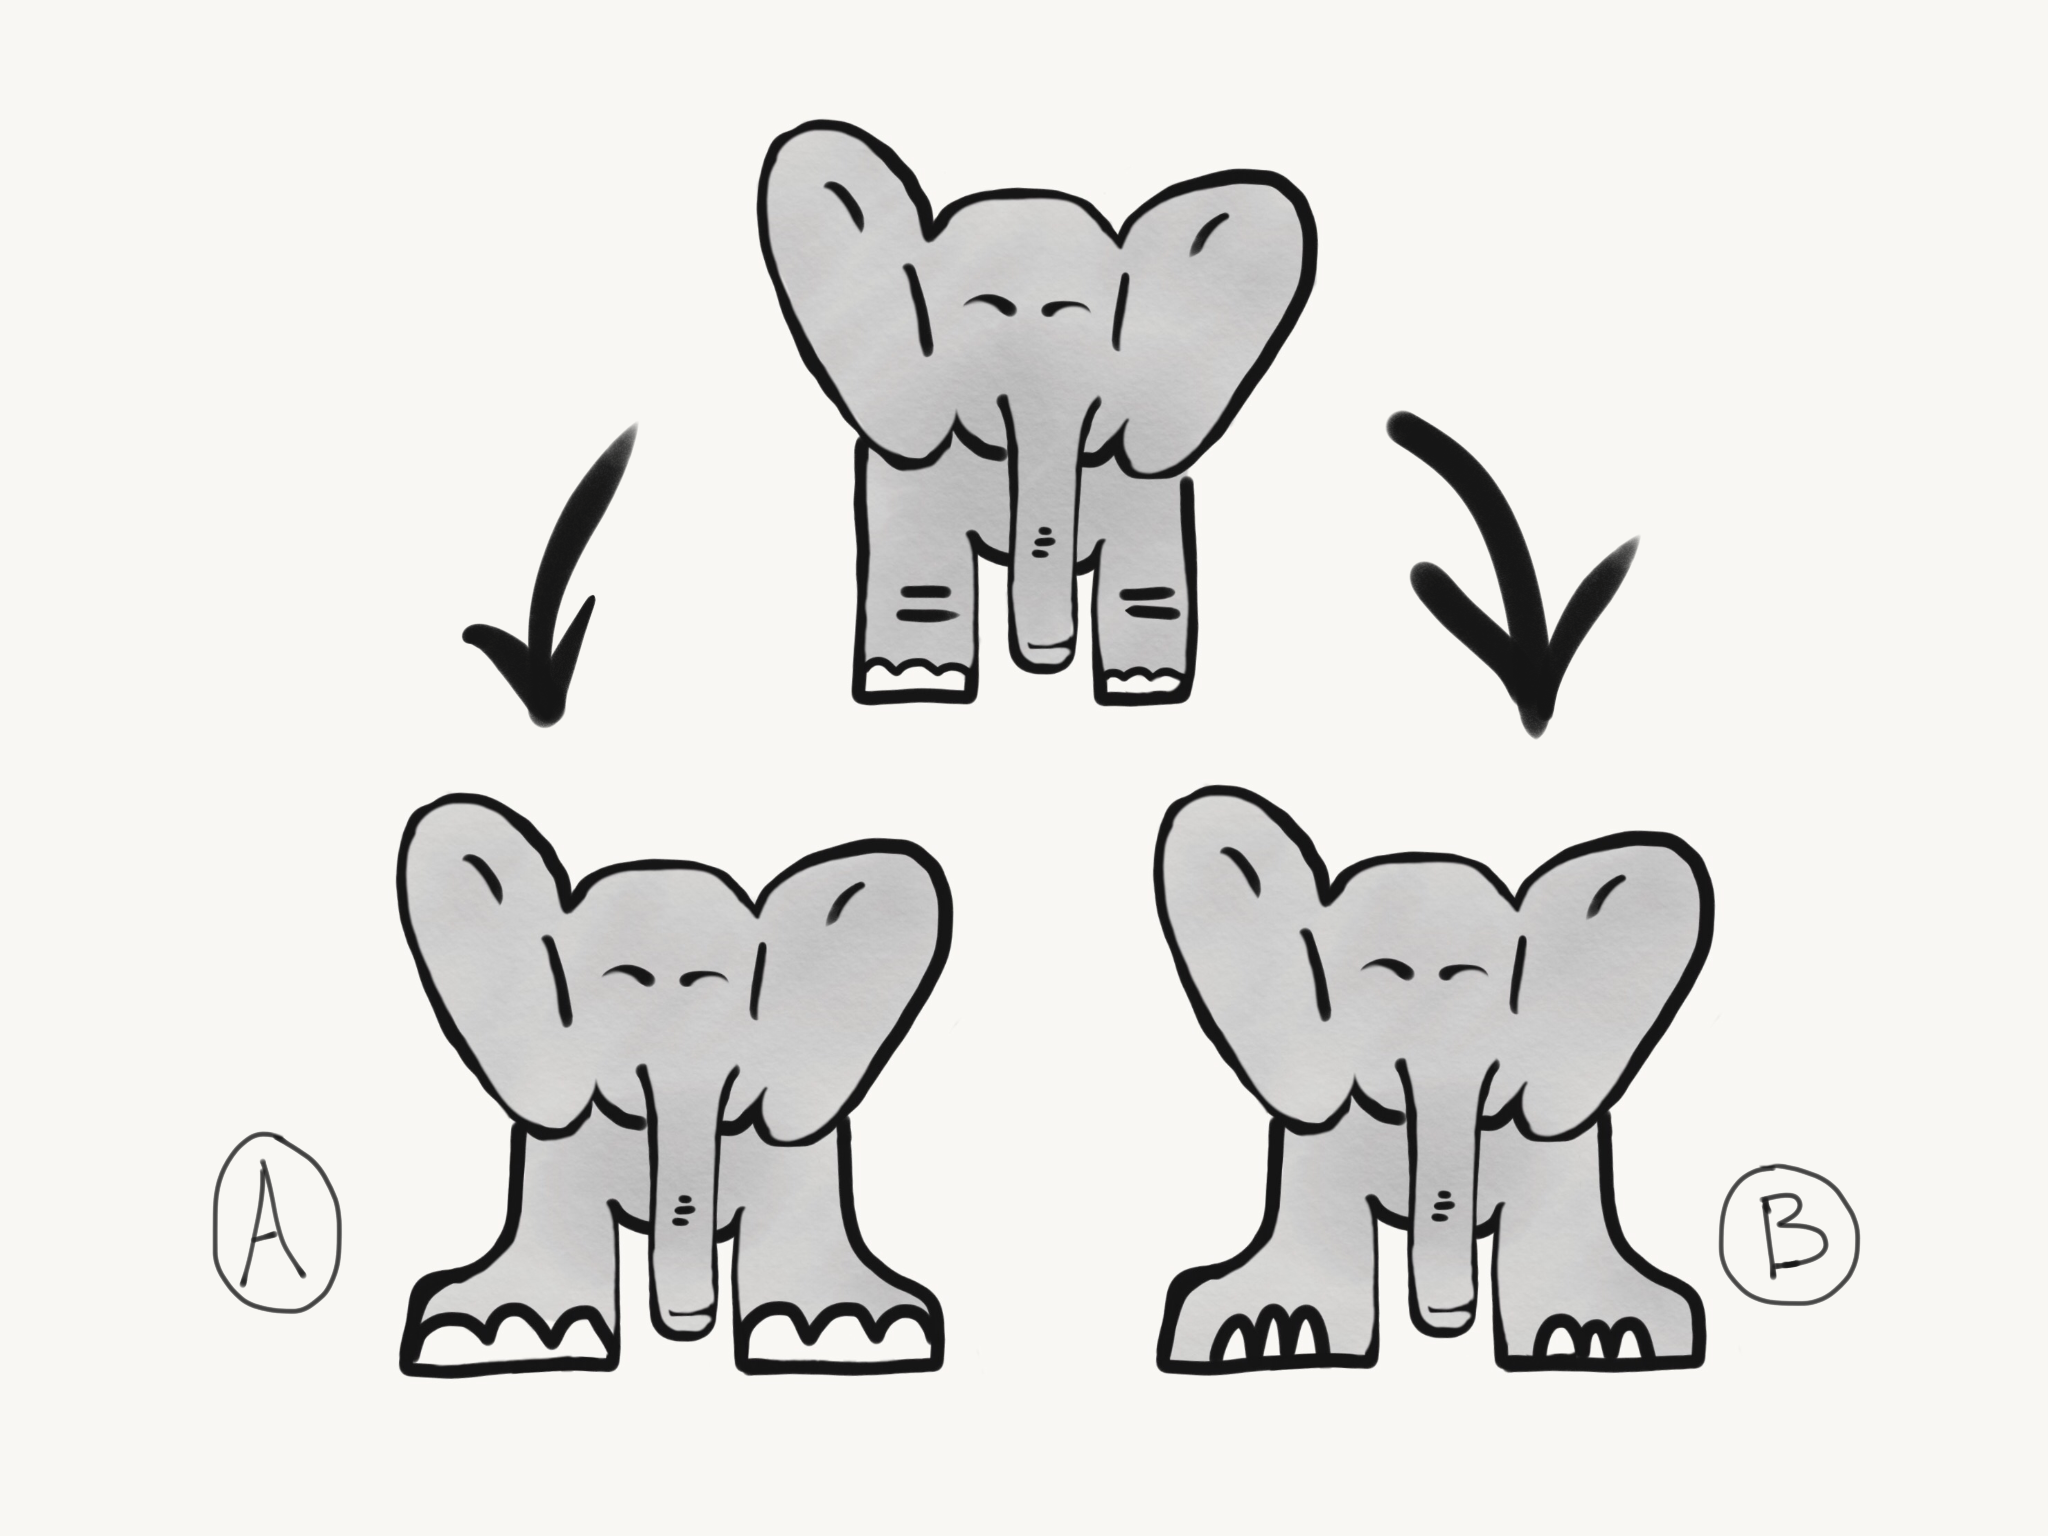
\includegraphics[width=0.8\textwidth]{img/exploratory_growth}
 	\captionsetup{singlelinecheck=off,justification=raggedright}
  	\caption{Illustration of exploratory growth; high evolvability left and low evolvability right \cite{Downing2015IntelligenceSystems}.}
    \label{fig:exploratory_growth}
\end{figure}
\end{frame}

\begin{frame}{Evolvability as Bias towards Useful Variation}
  \begin{figure}
    \centering
    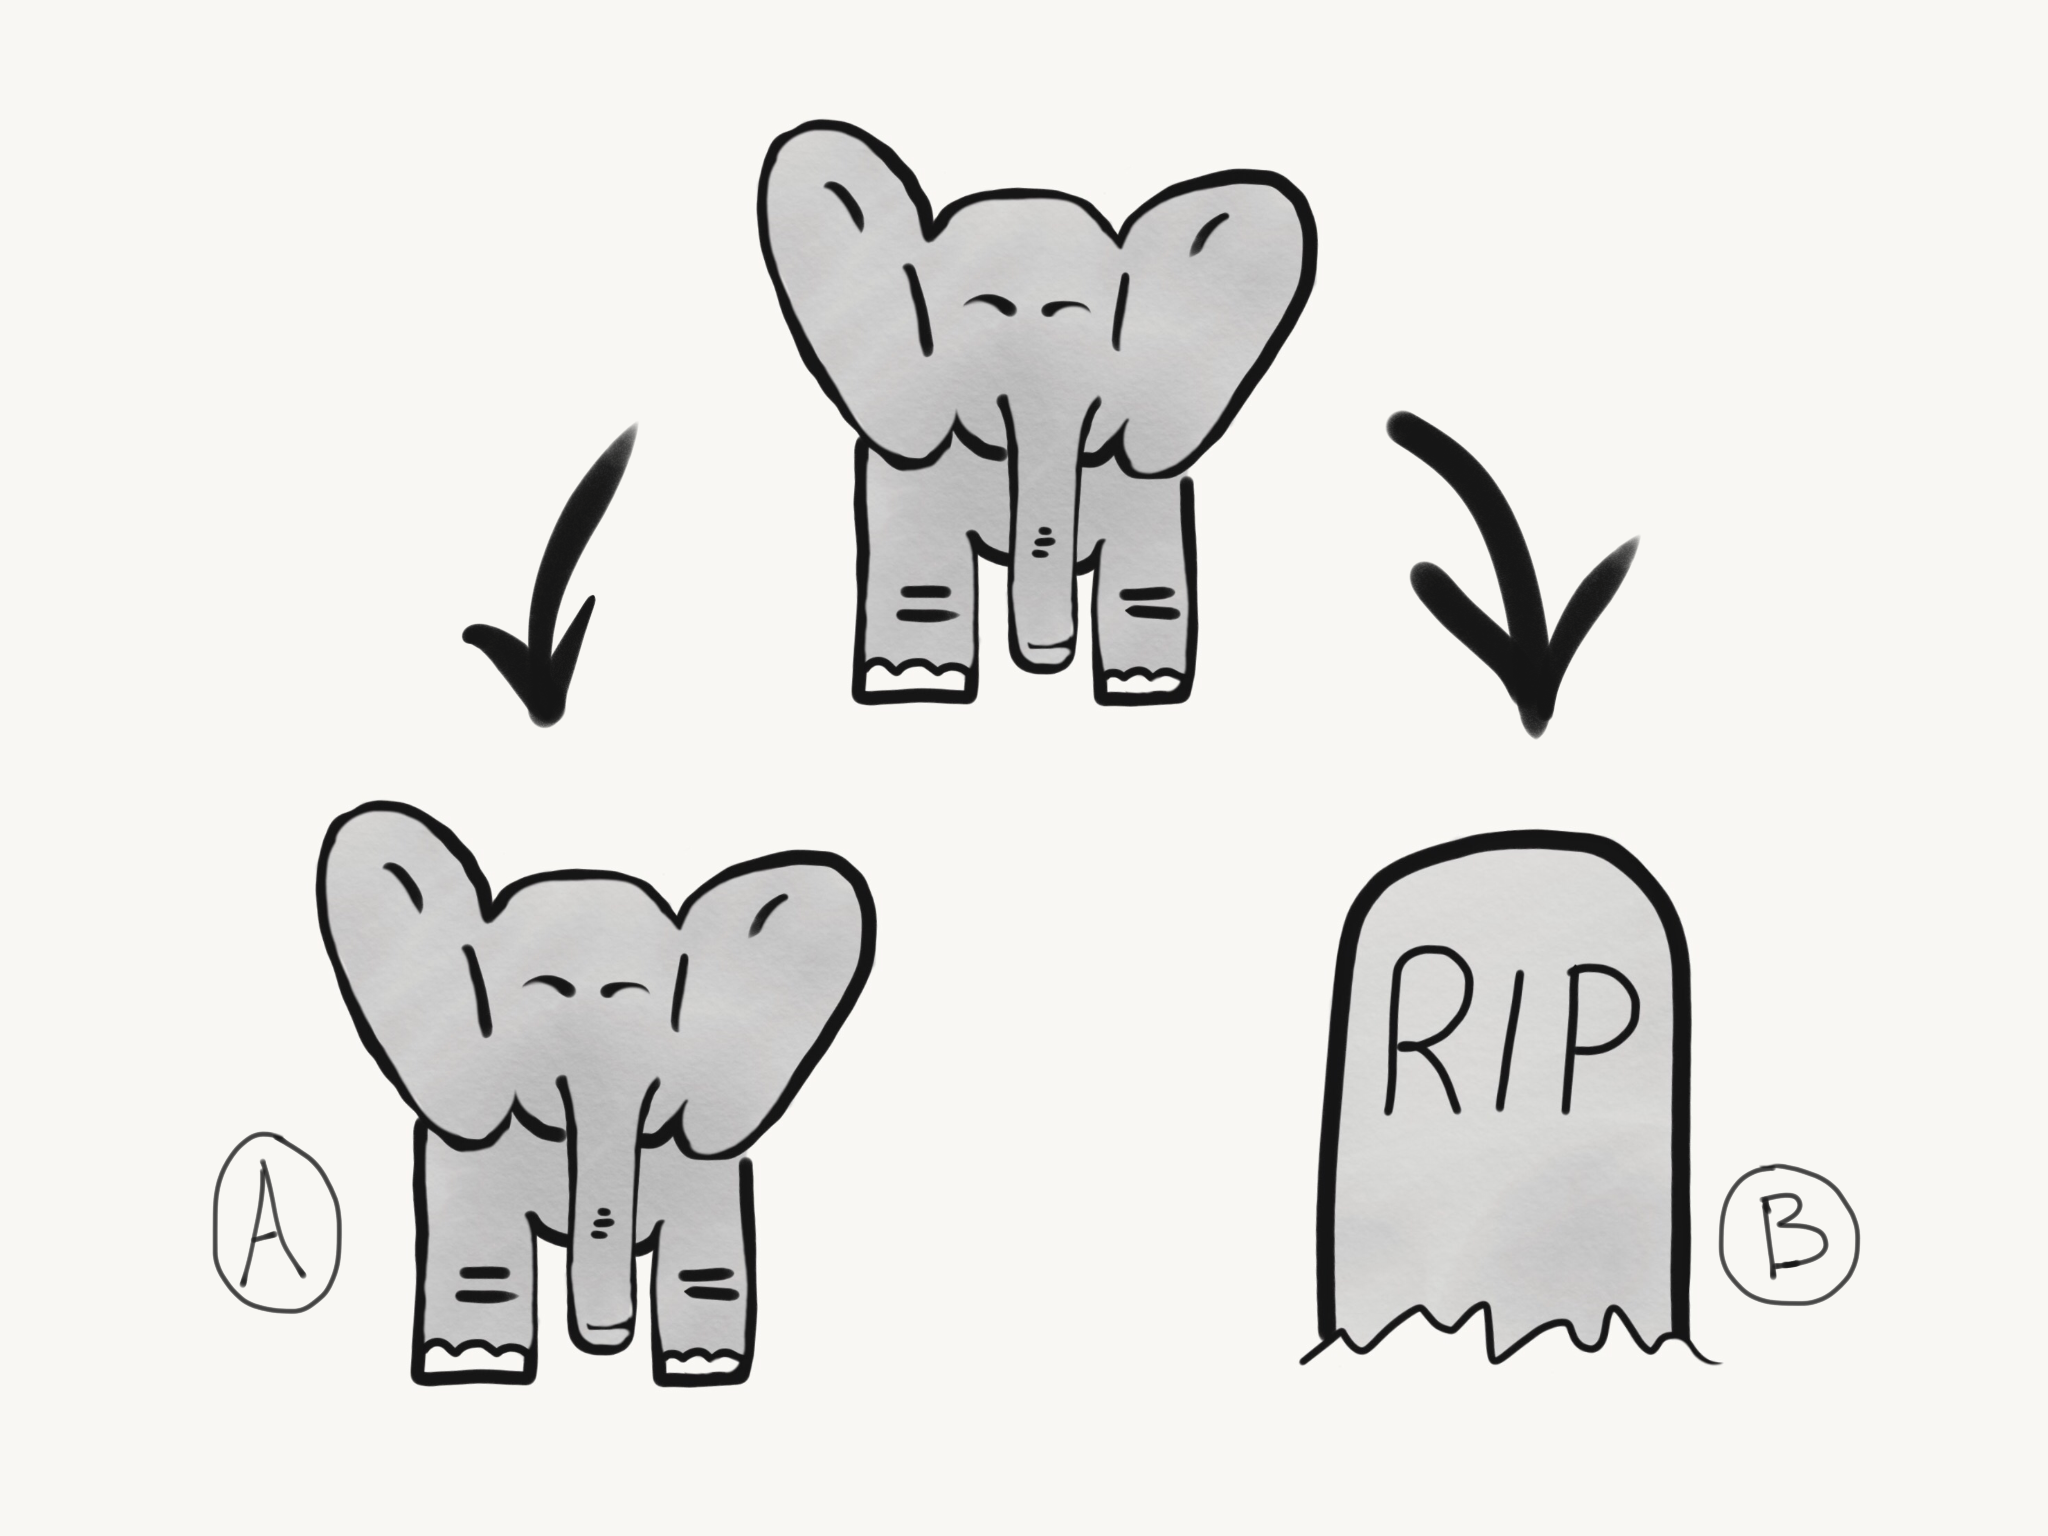
\includegraphics[width=0.8\textwidth]{img/robustness}
 	\captionsetup{singlelinecheck=off,justification=raggedright}
  	\caption{Illustration of robustness; high evolvability left and low evolvability right \cite{Downing2015IntelligenceSystems}.}
    \label{fig:robustness}
\end{figure}
\end{frame}
